\documentclass[../../main.tex]{subfiles}
\begin{document}

\begin{flushright}
  \footnotesize\textit{【自動文字起こし・要確認】}
\end{flushright}

[解 1] $A(t, 0), B(-t, 0) \; (t > 0)$ となるよう座標平面をとる．$P(x, y)$ とする．
$$ \overrightarrow{PA} =
\begin{pmatrix} t - x \\ -y
\end{pmatrix}, \quad \overrightarrow{PB} =
\begin{pmatrix} -t - x \\ -y
\end{pmatrix} $$
だから，
$$ |\overrightarrow{PA}| = \sqrt{(t - x)^2 + y^2}, \quad |\overrightarrow{PB}| = \sqrt{(t + x)^2 + y^2}, \quad \overrightarrow{PA} \cdot \overrightarrow{PB} = -(t^2 - x^2) + y^2 $$
となるので，与式に代入して，
\begin{align}
  & \sqrt{(t - x)^2 + y^2} \sqrt{(t + x)^2 + y^2} = c + t^2 - (x^2 + y^2) \\
  \iff & \left\{ (t - x)^2 + y^2 \right\} \left\{ (t + x)^2 + y^2 \right\} = \left\{ c + t^2 - (x^2 + y^2) \right\}^2 \\
  \iff &
  \begin{cases} \dfrac{x^2}{t^2 + \dfrac{1}{2} c} + \dfrac{y^2}{\dfrac{1}{2} c} = 1 & (\because c > 0, t > 0) \\ c + t^2 \ge x^2 + y^2
  \end{cases}
\end{align}
で，これを図示すると右図．よって，もとめる軌跡は
$$ \dfrac{x^2}{t^2 + \dfrac{1}{2} c} + \dfrac{y^2}{\dfrac{1}{2} c} = 1 $$

\begin{figure}[htb]
  \centering
  % 図示用に t=1, c=2 とし，楕円の長半径・短半径は sqrt(2), 1．
  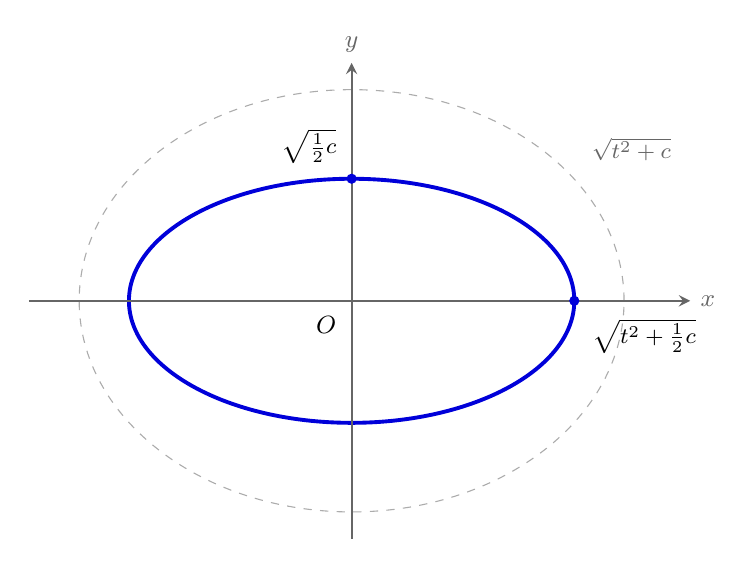
\begin{tikzpicture}[x=2cm, y=1.55cm, >=stealth, every node/.style={font=\small}]
    \draw[dashed, gray!65] (0,0) circle[radius=1.73];
    \draw[line width=1.4pt, blue!85!black] (0,0) ellipse[x radius=1.414, y radius=1];
    \draw[->, thick, gray!80!black] (-2.05,0) -- (2.15,0) node[right] {$x$};
    \draw[->, thick, gray!80!black] (0,-1.95) -- (0,1.95) node[above] {$y$};
    \node[circle, fill=blue!85!black, inner sep=1.3pt] at (1.414,0) {};
    \node[circle, fill=blue!85!black, inner sep=1.3pt] at (0,1) {};
    \node[below right=3pt, font=\footnotesize] at (1.414,0) {$\sqrt{t^2+\frac{1}{2}c}$};
    \node[above left=2pt, font=\footnotesize] at (0,1) {$\sqrt{\frac{1}{2}c}$};
    \node[above right=2pt, font=\footnotesize, gray!80!black] at (1.43,1.02) {$\sqrt{t^2+c}$};
    \node[below left=2pt] at (0,0) {$O$};
  \end{tikzpicture}
  \caption{条件を満たす楕円と，$x^2+y^2\leq t^2+c$ の境界円}
\end{figure}

[解 2] $|AB| = 2t, |PA| = a, |PB| = b, \angle APB = \theta$ とする．
$\triangle ABP$ が一直線上にない時，$\triangle ABP$ に余弦定理を用いて，
$$ 4t^2 = a^2 + b^2 - 2ab \cos \theta \cdots \text{①} $$
これは $A, B, P$ が一直線上の時 ($\theta = 0$) にも成立する．又，与式から，
$$ ab (1 + \cos \theta) = c $$
$$ \therefore ab \cos \theta = c - ab $$
①及び $-1 \le \cos \theta \le 1$ に代入して，
\begin{align}
  & 4t^2 = a^2 + b^2 - 2(c - ab) = (a + b)^2 - 2c \\
  \iff &
  \begin{cases} a + b = \sqrt{4t^2 + 2c} & \cdots \text{②} \\ c \le 2ab & (\because a, b, c \ge 0) \cdots \text{③}
  \end{cases}
\end{align}

\begin{figure}[htb]
  \centering
  \begin{tikzpicture}[x=2.1cm, y=1.7cm, every node/.style={font=\small}]
    \coordinate (B) at (0,0);
    \coordinate (A) at (2.3,0);
    \coordinate (P) at (1.35,1.45);
    \draw[line width=1.3pt, blue!85!black] (B) -- (P) -- (A) -- cycle;
    \node[circle, fill=blue!85!black, inner sep=1.3pt] at (B) {}; \node[circle, fill=blue!85!black, inner sep=1.3pt] at (A) {}; \node[circle, fill=blue!85!black, inner sep=1.3pt] at (P) {};
    \node[below left=2pt] at (B) {$B$};
    \node[below right=2pt] at (A) {$A$};
    \node[above=2pt] at (P) {$P$};
    \node[left=3pt] at (0.6,0.72) {$b$};
    \node[right=3pt] at (1.85,0.72) {$a$};
    \node[below=7pt] at (1.15,0) {$2t$};
    \draw[orange!85!black, thick] ($(P)+(-0.17,-0.25)$) arc[start angle=235, end angle=315, radius=0.3];
    \node[below=5pt, orange!85!black] at (P) {$\theta$};
  \end{tikzpicture}
  \caption{$AB=2t$, $PB=b$, $PA=a$, $\angle APB=\theta$}
\end{figure}

②が [解 1] の座標平面で表すのは，原点を中心，長半径 $\dfrac{1}{2}(a+b) = \sqrt{t^2 + \dfrac{1}{2} c}$, 短半径 $\sqrt{t^2 + \dfrac{1}{2} c - t^2} = \sqrt{\dfrac{1}{2} c}$ の
楕円: $\dfrac{x^2}{t^2 + \dfrac{1}{2} c} + \dfrac{y^2}{\dfrac{1}{2} c} = 1$ である．この時 $a+b=A$ とすると $\dfrac{A}{2} - t \le a \le \dfrac{A}{2} + t$ で
$$ ab = a(A - a) \ge \left( \dfrac{A}{2} - t \right) \left( \dfrac{A}{2} + t \right) = \dfrac{A^2}{4} - t^2 = \dfrac{1}{2} c \quad (\text{等号成立は } a = \dfrac{A}{2} \pm t) $$
で，③は常に成立．したがって，もとめる軌跡は
$$ \dfrac{x^2}{t^2 + \dfrac{1}{2} c} + \dfrac{y^2}{\dfrac{1}{2} c} = 1 $$
となる．

\end{document}
